\documentclass[12pt,a4paper]{article}

\usepackage[english]{babel}
\usepackage{hyperref}
\usepackage{graphicx}
\usepackage{nicefrac}
\usepackage{caption}
\usepackage{wrapfig}

%% The title of your survey
\title{ Survey of mobile network security in trending technologies, focusing on Bluetooth and NFC }

%% Both authors
\author{ Johannes Kurz \\
         e0727957 \\%student ID
         \and
         Gerhard Schraml \\
         e0728067 % student ID
}
\date{\today}

%% The actual contents of the document
\begin{document}

%% Generate the title
\maketitle

%% Write the abstract  
%% ----------------------------------------------------------------------------
\begin{abstract}
\noindent
Write a short abstract about the topics contained in the paper. This is usually the last step to do.
\end{abstract}


%% Introduction
%% ----------------------------------------------------------------------------
\section{Introduction}

\begin{table}
\begin{tabular}{r|l}
\hline
\multicolumn{2}{c}{paper structure proposal} \\
\hline
1 - 1\nicefrac{1}{2} page & title + abstract + introduction \\
1 page & mobile networks security basics general \\
\nicefrac{1}{2} page & nfc general description \\
\nicefrac{1}{2} page & nfc threat introduction and listing \\
3 - 5 pages & nfc threats in detail (1 page per threat?) + solution \\
4 - 6 pages & bluetooth TODO shorty \\
\nicefrac{1}{2} page & conclusion \\
1 - 2 pages & references \\
\hline \hline
11\nicefrac{1}{2} - 17 pages & total \\
\hline \hline
\end{tabular}
\end{table}

What you should include in the introduction
\begin{itemize}
 \item Describe the topic (Importance, Significance)
 \item Give a summary of the surveyed topic
\end{itemize}


%% Actual Survey Work
%% ----------------------------------------------------------------------------
%% You can introduce further sections as well
\section{Mobile Networks Security Basics General}
Mobile Networks are all around us. Starting from basic GSM cellphone networks to special applications like payment using near field communication technology. In this survey we want to introduce two technologies and discuss their security concepts, flaws and exploits.

\section{Security in Near Field Communication}

\subsection{Terms and general description}

More and more people world wide start using \emph{Near Field Communication} (NFC) for personal purposes. Goal of the technology is the convenient transfer of small amounts of data by just simply wiping compatible devices over each others. As the communication is contactless, bringing sender and receiver to close proximity suffices to establishing a connection. Usually the working distance for NFC connections does not exceed about 10 to 20 centimeters. The technology is based upon \emph{Radio-Frequency Identification} (RFID) - it 	similarly uses electromagnetic radiation for transporting signals over small distances. Therefor a small magnetic field is established with the purpose of bridging the physical space between participating devices.

Basically two types of NFC devices exist. \emph{Active devices} take care of the establishment of the necessary magnetic field. As this is an energy-consuming task, they are usually connected to a power supply. \emph{Passive devices} normally don't possess a built-in power supply. They make use of small amounts of power they are able to harvest from the magnetic field issued by a connected active device. Hence, passive devices are idle when there is no connection present. Typical examples for such devices are so-called NFC tags, e.g. containing additional information about an exhibit in a museum where it is attached to. A user could then easily access this information by hovering its NFC-enabled electronic device, capable of reading the NFC tag, over it.

Mobile devices can choose out of three different communication modes. In \emph{Peer-To-Peer} mode, two active NFC-enabled devices communicate on an equal basis. Usually the task of emitting the necessary magnetic field is carried out in an alternating way by both participants. In \emph{Reader/Writer} mode an active device is reading data from respectively writing data to passive NFC tags. Finally, in \emph{Card Emulation} mode a mobile device is acting as NFC tag allowing other (active) devices to read information from it. This mode is mostly used for electronic ticketing or contactless payment applications using mobile phones.

\subsection{Smart Poster Spoofing}

Typically, NFC communication between mobile devices and tags (or other devices) uses the \emph{NFC Data Exchange Format (NDEF)}. It is defined by the NFC Forum\footnote{\url{www.nfc-forum.org}}, a standardization organisation in the area of NFC. The NDEF format consists of several record data types, headed by \emph{Text}, \emph{URI} and \emph{Smart Poster} record types.\cite{DBLP:conf/IEEEares/Mulliner09}\cite{DBLP:conf/mobisys/GummesonPGTZ13}

Text records simply contain an arbitrary, human-readable text, optionally followed by a language identifier.

URI records include a URI of arbitrary protocol pointing to further information or an action to perform. Based on the protocol, e.g. HTTP, TEL, SMS, MAILTO, the receiving device determines the target application to deal with the given URI. Thus the NFC subsystem of a device can be seen as kind of a job dispatcher.

Smart Poster records usually consist of a text record, containing the title or short description of a hovered NFC tag, and a URI record pointing to some more detailed information on the item the tag is attached to. One proper use case is, as already mentioned above, to provide further information on museum exhibits by just hovering the attached NFC tag.

\subsubsection{Manipulating the content of a Smart Poster}

In \cite{DBLP:conf/IEEEares/Mulliner09}, a way of tricking users into acknowledging actions, they actually don't want to perform, is presented. One could physically replace smart tags with new ones containing malicious information. Due to limitations of a smart phone device, expected information is shown at the display of a victims device, while the underlying action e.g. links to an attackers site. In the test, a Nokia 6131 device was used, which would display only the text content of a Smart Poster if it exceeds the screen size. Thus, the transported URI is, at least at first sight, not presented to the user. Figure \ref{img_smart_poster_spoofing} shows an example of how such a spoofed message could be constructed. Another example is the abuse of the TEL protocol issuing a phone call. The attacker could display a trusted phone number while actually attaching a premium rate number leading to unwanted expenses for the victim.

\begin{figure}
\begin{center}
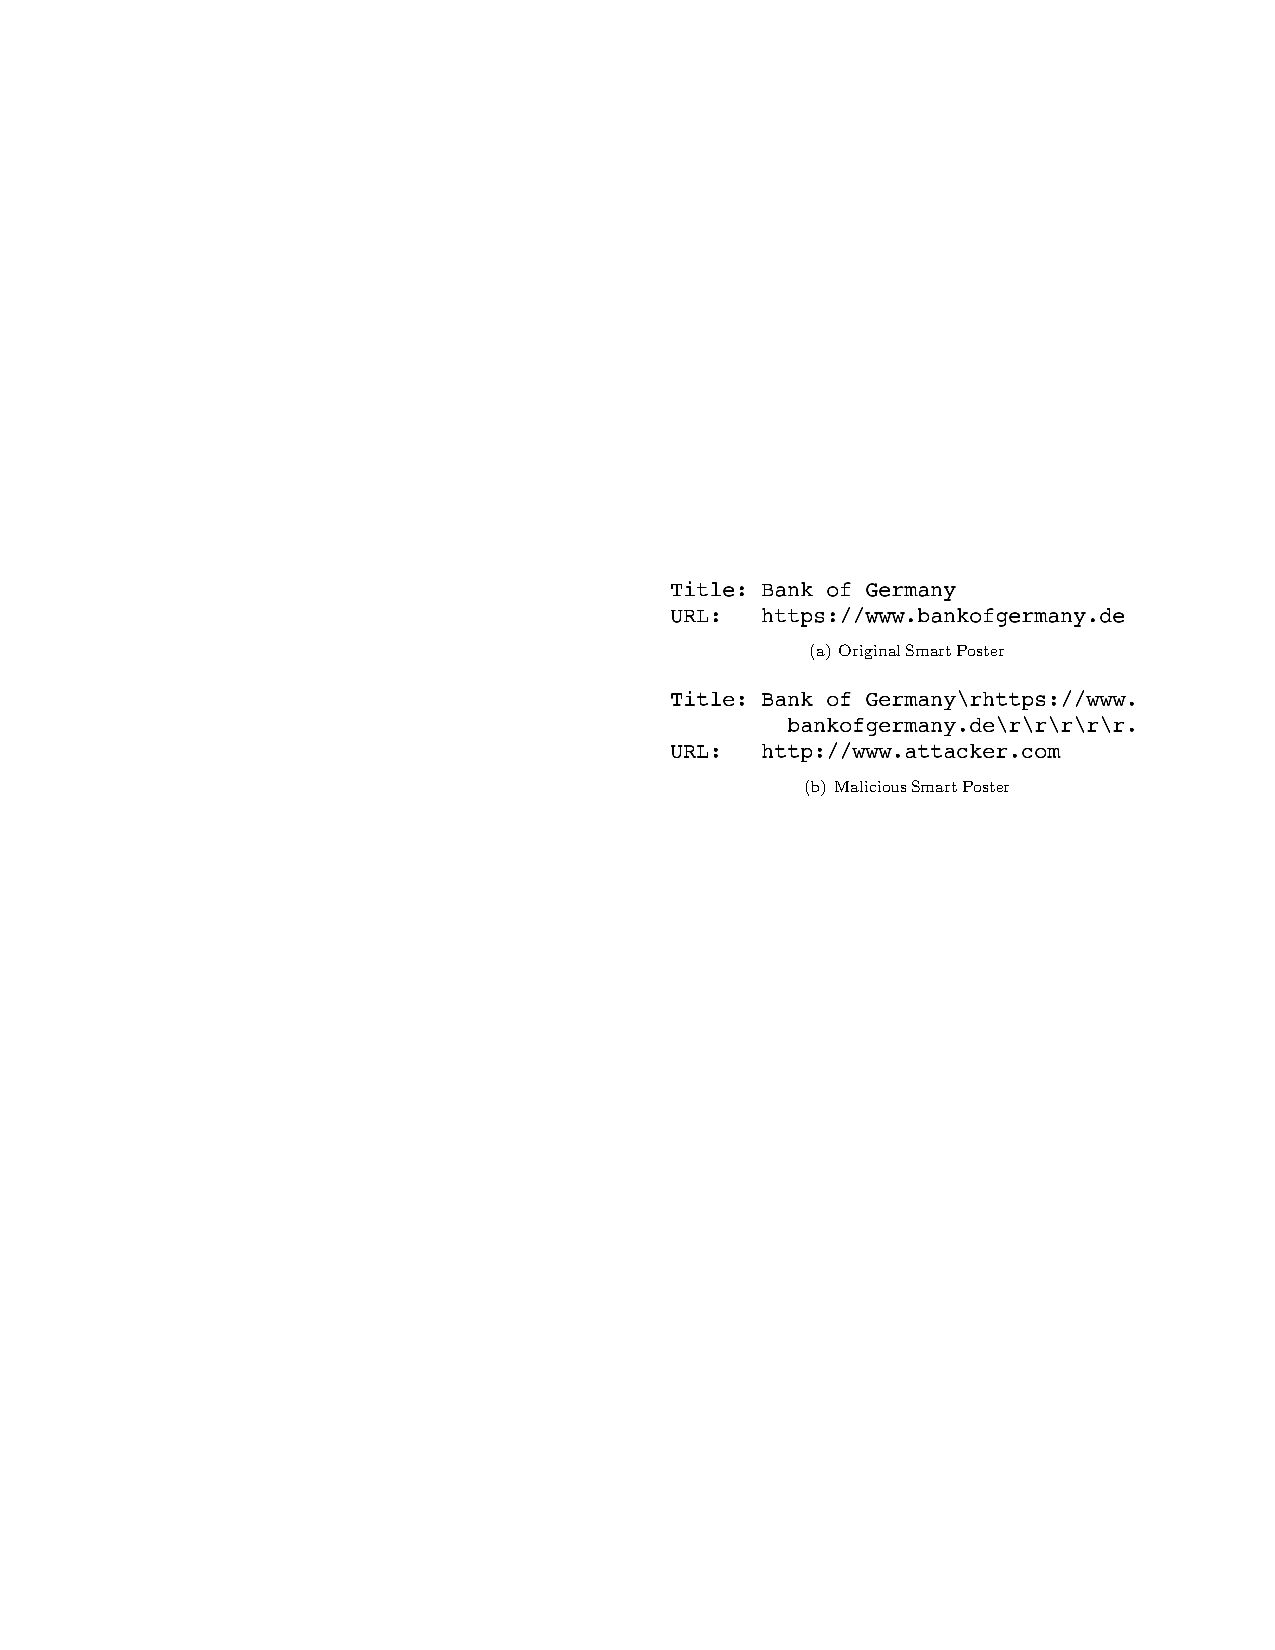
\includegraphics{img/smart_poster_spoofing}
\caption{\footnotesize{Smart Poster Spoofing Example\cite{DBLP:conf/IEEEares/Mulliner09}}}
\label{img_smart_poster_spoofing}
\end{center}
\end{figure}

\subsubsection{Countermeasures against Smart Poster Spoofing}

\paragraph{Verifiying data trustworthyness via online backend}
\cite{DBLP:conf/wowmom/WuQKKT12} presents S-SPAN, a system aiming at securing the use of Smart Poster reads from NFC tags. Basic approach is not to store the actual information in plain text on the NFC tag. The tag rather contains a non-guessable and non-human-readable identifier which is used to locate the Smart Poster contents in an online database. The user of the mobile device has to be logged into the online database when touching the NFC tag. Over secured connection, the database is queried for the identifier and replies with the actuals contents. The contents of the database are administered by the owner of the smart tag. Identifiers are never used twice to prevent accidental reusage of already expired tags. Consequently, Smart Poster can expire at some time. The approach entails better security as actual URIs are always retrieved by a trusted entity. On the other hand, additional latency has to be accepted for querying the database.

\paragraph{Verifying data trustworthyness via local middleware}
\cite{DBLP:conf/trustcom/HameedHHK14} refers to the latency problem of S-SPAN and presents a "Lightweight Security Middleware to Detect Malicious Content in NFC Tags or Smart Posters". The proposed middleware is run between the NFC controller and the application layer of the device and takes care of all Smart Poster tag reads. In contrast to S-SPAN, data (Text and URI) is directly stored on the tag. The middleware, depicted in figure \ref{img_lightweight_security_middleware}, performs a series of checks against the delivered URI. First, a \emph{white list} is queried against the URI. If the given URI can be found, the Smart Poster is directly forwarded to the application layer. If not, a \emph{black list} approach is performed. If the URI is blacklisted, the middleware prompts the user to decide on whether to continue reading the Smart Poster. If the URI is not blacklisted, a final validation attempt is made by querying \emph{Crowd-sourced Internet Website Reputation Ratings}. When the query results in a predefined minimum reputation score, the Smart Poster again is forwarded. Performance observations show, that white- and blacklist hits cause very low latency, while reputation querying takes a maximum of 1 second in the given test environment.

\begin{figure}
\begin{center}
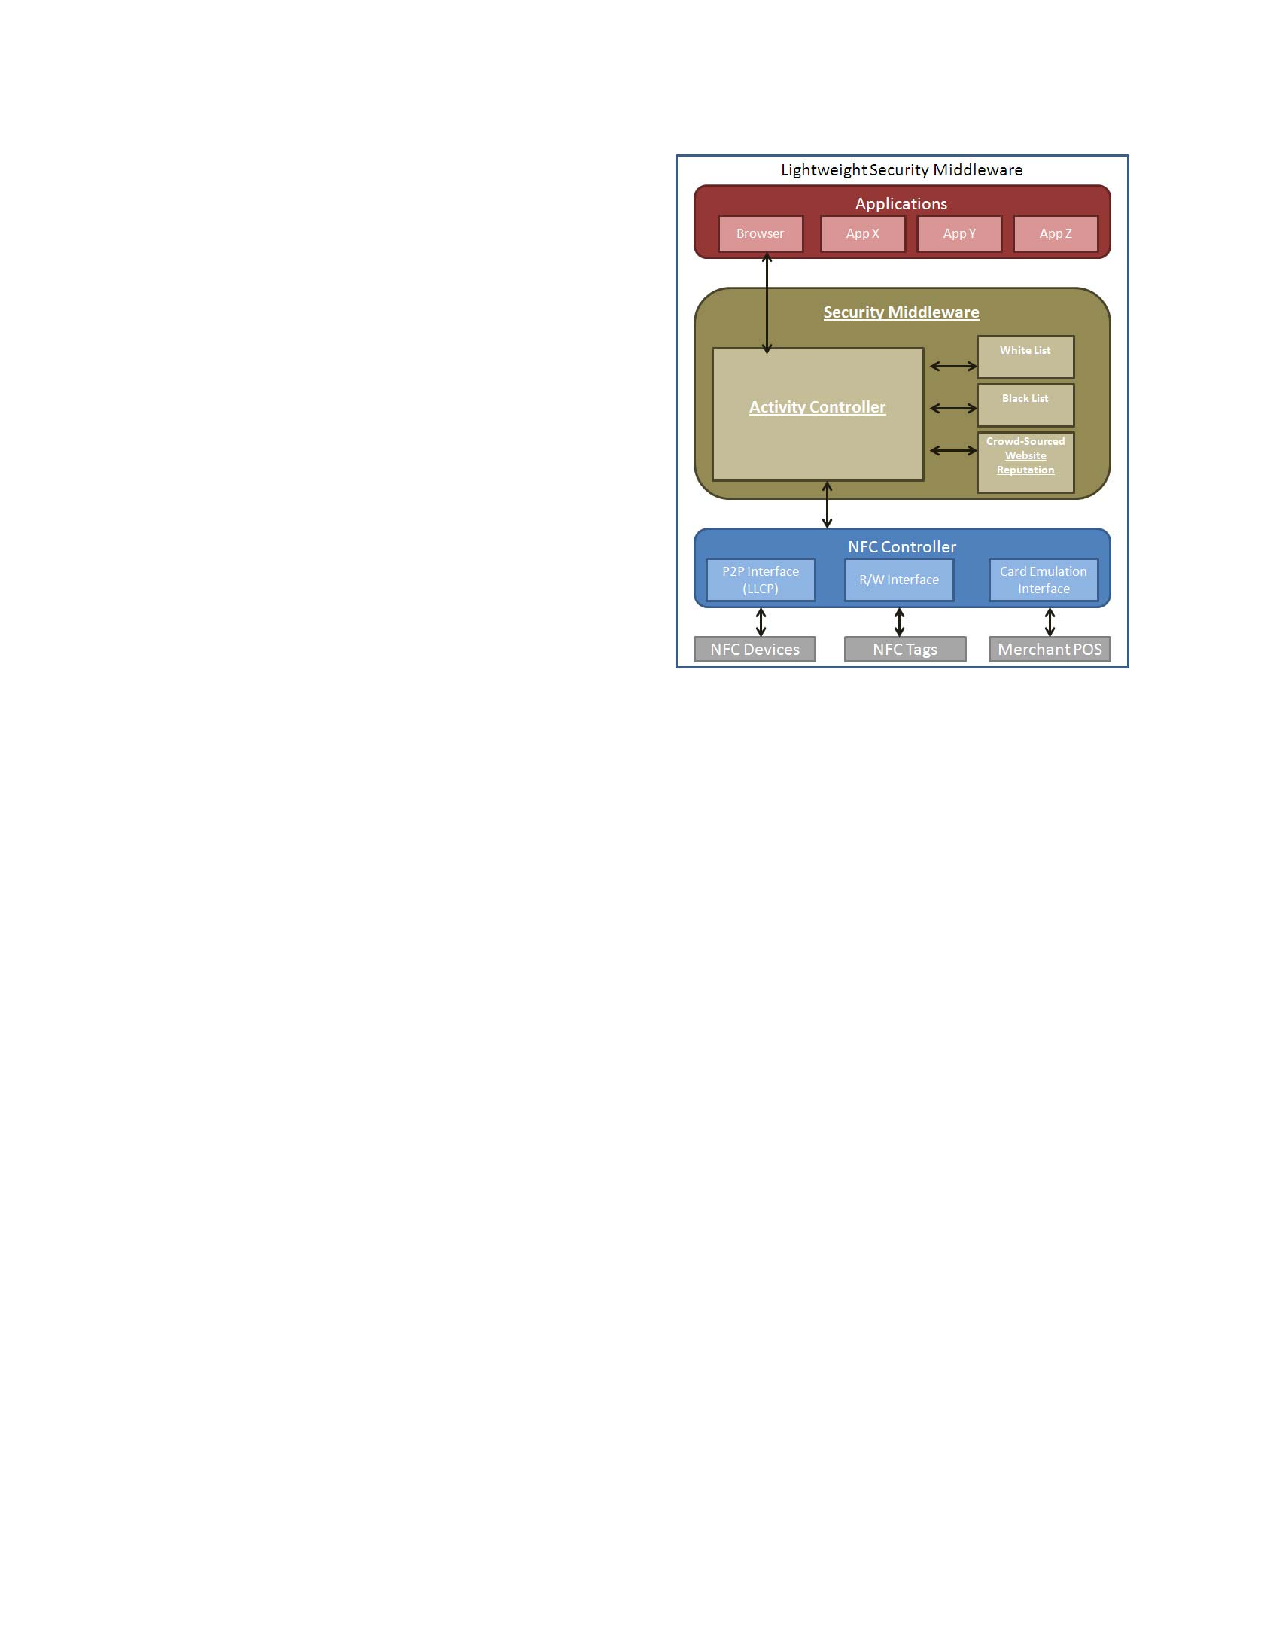
\includegraphics{img/lightweight_security_middleware}
\caption{\footnotesize{NFC application architecture from \cite{DBLP:conf/trustcom/HameedHHK14}}}
\label{img_lightweight_security_middleware}
\end{center}
\end{figure}

\paragraph{Preventing untrusted data from being received by signal jamming}
While the previously presented countermeasures use device-internal verification of received data, \cite{DBLP:conf/mobisys/GummesonPGTZ13} proposes an external approach by attaching a credit card-sized module called \emph{EnGarde} at the back of an NFC device, similar to \emph{nShield}\cite{DBLP:conf/mobisys/ZhouX14}. The main purpose of \emph{EnGarde} is to detect malicious NFC data before it is fully perceived by the device and immediately start jamming the signal in order to letting the whole transmission fail. 

The detection of unwanted or manipulated messages uses a programmable, rule-based approach. As a result, messages of specific (1) \emph{protocols}, (2) \emph{tag identifiers} or even (3) \emph{message content} can be blocked.

(1) The identification of the present protocol starts with an examination of the first pulse of the AM carrier of a message. After gaining a first grouping by this step, a lightweight algorithm is deployed to exactly identify the used protocol by having a quick look at the first bytes of the sniffed transmission. Practically, protocol prohibition can be used for e.g. avoiding all communications over the ISO-14443-A protocol, which can be used to read out a devices NFC identifier.

(2) Tag identifiers can also be sniffed at an early phase of the connection, the so-called anti-collision phase. Consequently, blacklisted tags or even whole families of tags (e.g. from a certain manufacturer) can be blocked.

(3) Using a software graph structure, connections can even be blocked by specific contents of a message, which occurs to be the finest granularity of blocking rules. Considering the above-discussed NDEF data exchange format, messages containing particular blacklisted URI records (e.g. all URIs starting with ``http://www.evil.com") can be blocked.

The concrete implementation of signal jamming is based on the type of NFC connection. For tag-to-reader communications \emph{reflective jamming} is used, which basically generates a subcarrier of same frequency of the NFC subcarrier (i.e. 847.5kHz) using load-based modulation of the tuned coil. In contrast, for interrupting incoming active NFC communications, so-called \emph{pulse jamming} is introduced, which unfolds its destructive power by generation of targeted pulses. Both jamming techniques work at very low power consumptions.

\subsection{Eavesdropping Near Field Communication}

Eavesdropping, ``to listen secretly to the private conversation of others"\footnote{\url{http://www.thefreedictionary.com/eavesdrop}}, concerns almost any forms of transmission of digital data. Obviously, wireless connections are particularly vulnerable to being intercepted by third persons, and so NFC connections are. \cite{DBLP:conf/icitst/EvestiSS13}

Despite the general opinion that the operating distance of NFC is too short for the possibility of eavesdropping attacks, recent research suggests to keep it definitely in mind. Although the working distance does usually not exceed 10 to 20 centimeters, many devices emit NFC signals at much higher strength as necessary. In \cite{DBLP:conf/mobisys/ZhouX14} it is proved that in some cases transmissions can be intercepted within up to a range of 240 cm. This is at least more than an order of magnitude in comparison to the above-mentioned intended operating distinace of few centimeters, which probably suffices for performing serious attacks.

\subsubsection{Countermeasure: Signal attenuation}

The authors of \cite{DBLP:conf/mobisys/ZhouX14} propose a hardware-level solution. As current NFC chipsets use fixed transmission power, device-internal solutions are difficult to find. Thus, \emph{nShield} is introduced, which is basically an electronic element of credit card-size, to be attached at the back of the NFC device. The elements purpose is to attenuate the device-provided radio-frequency field, if it is too strong. One of the challenges of this approach is, that different devices issue their RF fields in different strengths. Thus, a fixed attenuation factor probably would lead to unsatisfactory results. Therefor, an adaptive RF field strength regulation is designed, which ensures the sufficiency of the emitted signal strength and prohibits signal loss.

\emph{nShield} basically consists of two components. First, a software-defined passive NFC radio-platform, capable of receiving and transmitting data. The platform uses its antenna for attenuating signals as well as for harvesting energy from the emitted RF field of the device it is attached to. By rectifying the RF signal to a DC voltage and the following regulation of the voltage a 20mAh on-board battery is charged. The energy harvested in this manner is sufficient for ensuring permanent power supply for the component. Thus, an external power supply is not necessary.

\begin{quote}
``nShield reduces the risk of eavesdropping by absorbing the excessive RF power radiated by the initiator with an adjustable attenuator, which is multiplexed with the load modulator."\cite{DBLP:conf/mobisys/ZhouX14}
\end{quote}

The second important component is the algorithm used for the adaptive RF field attenuation. An embedded TX control circuit ensures strictly timed data transmissions in a synchronized manner based on the data rate of the used modulation scheme. After extracting the raw transmission data by removing the AM carrier and demodulating the baseband signal, the optimal transmission power of the initiator is computed. Therefor the successful reception of previous messages is derived by analyzing logical relations between consecutive messages. Binary search is used to accelerate this step.	If no RF field is present, the component falls asleep to conserve power.

%Figure \ref{img_nshield} shows a prototype compilation of the necessary hardware components, attached to a Google Nexus 7 tablet. While the size of the circuit board is 5.5 cm by 5.3 cm, the antenna measures 9.6 by 9.6 cm. The components could be shrinked further without loss of functionality to fit smaller mobile devices. Component cost is specified with under \$20.

%\begin{figure}
%\begin{center}
%\includegraphics{img/nshield}
%\caption{\footnotesize{Antenna and circuit of \emph{nShield} mounted on the back of a Google Nexus 7 tablet\cite{DBLP:conf/mobisys/ZhouX14}}}
%\label{img_nshield}
%\end{center}
%\end{figure}

Experimentation results with the prototype show a mean delay due to the attenuation process of 2.1 seconds, measured from the very first probe transmission to the point in time the optimal attenuation level is determined. It is also shown that, using simple aluminium foil to reduce the strength of the RF field of an initiator, the maximum passive eavesdropping distance can be reduced to about 80 centimeters without affecting the reliability of connection. However, a concrete comparison of eavesdropping distances without/with \emph{nShield} attached to a NFC device is somehow missing.

\subsubsection{Countermeasure: Signal jamming}



TODO denial of service? = basically just jamming the signal - from the attackers point of view

bar bar foo foo

\subsubsection{TODO: Software countermeasure?}

Software level: TODO maybe find a solution to NFC eavesdropping at software level?


\subsection{Relay attacks}

TODO man-in-the-middle? more general than relay attacks?

Problem description, practical implementations and countermeasures \cite{DBLP:journals/compsec/HanckeMM09} \cite{DBLP:conf/rfidsec/FrancisHMM10} \cite{DBLP:conf/sec/RolandLS12}

bar bar foo foo

\section{Security in Bluetooth communications}
\subsection{Terms and general description}
\begin{wrapfigure}{r}{0.5\textwidth}
  \begin{center}
    
\includegraphics[width=0.48\textwidth]{img/730px-Bluetooth-Logo.png}
  \end{center}
  \caption{Bluetooth logo with the combined initial letters (runes) of King Harald "Bluetooth" Gormsson}
  \label{img_bt_logo}
\end{wrapfigure}
The technology behind Bluetooth (BT) was developed in the early 1990s and commercial successful after the millennium. With the integration in the main stream devices and Microsoft Windows (XP SP1 2001) security flaws started to pop up. Similar to NFC bluetooth is a radiation based communication technology for one to seven devices. Bluetooth devices can have master or slave role and with these operation role. The range and used technology on the other hand differ as described later. 
Bluetooth has a broad variety of use cases from headsets, input devices, gaming consoles, industry networks, cars and even medical equipment like a pacemaker. At the \emph{Chaos Computer Congress 2007} (CCC) there was a talk about "Hacking the Bionic Man" \footnote{\url{http://events.ccc.de/camp/2007/Fahrplan/events/2049.en.html}} including Bluetooth attacks. Therefore not only smartphones cars and our computers are vulnerable to attacks.
The topic is not new but still relevant. Recent applications are wearables like fitness wristbands or watches. With everyone owning a BT enabled notebook, smartphone, car or already a smartwatch this targets most people. \\
Bluetooth uses the (ISM) band at 2.4 to 2.485 GHz and is distinguished in three classes and four versions. The first class uses a power of 100mW and has a range of about 100m. The second class uses 2.5mW with a range of 10 meter. The third class uses only 1mW with a range of about 1m.\\
The four different versions introduced new features and higher data rates. In version 2.0 the \emph{Enhanced Data Rate} (EDR) was introduced. Currently version 4.0 from 2010 has a data rate of 24 Mbit/s (in 3.0 over a colocated 802.11 link). Additionally 4.0 introduced \emph{Bluetooth low energy} (Bluetooth LE, BLE) to be run from a coin cell power source. The latest version 4.2 was released on December 2, 2014 introducing key features for the \emph{Internet of Things} (IoT).\\
The above list is not nearly exhaustive because with every version different protocols, security standards, power control mechanisms and many other features were added. In the following section the used or exploited technologies will therefore be briefly introduced and discussed.

\subsection{Bluetooth Security}
In this section the security concepts will be discussed including modes, key management, authentication, encryption and trust levels. Furthermore executable attacks and risk analysis in the case of a Automotive Environment (A-ENV) will state the realized or realizable possibilities. Last part will be the current state in the expanding applications of Low Energy Bluetooth technology. Therefore the referenced papers were classified in three categories: 
\begin{itemize}
	\item Basic technology risks
	\item Executable attacks and risks in case of A-ENV
	\item LE Bluetooth security concerns
\end{itemize}


\subsubsection{General concept}
%TODO: \cite{DBLP:journals/ijnsec/YehPWH12} \cite{DBLP:journals/ijnsec/Lackner13}  \cite{DBLP:conf/apnoms/FanSL11}

\textbf{Bluetooth Pairing} in versions below 2.1 a pin was used to authenticate between devices and then generate a link key and a encryption key for data transfer. The biggest problem with that was that when having the pin (or cracking) one can calculate the link key of the previous session and read all captured data. With version 2.1 the SIG (Special Interest Group) introduced the \emph{Secure Simple Pairing} (SSP) wich uses public-private key pairs to overcome the generation of the link key by pin guessing \cite{DBLP:conf/apnoms/FanSL11}. SSP has four stages described in \cite{DBLP:conf/apnoms/FanSL11},  \cite{DBLP:journals/ijnsec/YehPWH12} and in detail in \cite{DBLP:journals/ijnsec/Lackner13} :

\begin{itemize}
	\item \textbf{Key Exchange:} Generation of Elliptic Curve Diffie-Hellman Key (DHKey) pairs and exchange of public keys.
	\item \textbf{Authentication Stage 1:} exchange of parameters using one of four protocols (Numeric Comparison-, Out of Band,- Passkey Entry Protocol and Just Works only stated in  \cite{DBLP:journals/ijnsec/Lackner13})
	\item  \textbf{Authentication Stage 2:} sending messages to check for complete parameters and values
	\item  \textbf{Link Key Generation:} actual Link Key (LK) computation based on a function using previous exchanged parameters
\end{itemize}

There is a discovery phase and there may be addition or less steps depending on the Encryption mode which was chosen. Mode 1 provides no encryption (early BT versions). Mode 2 provides direct communication encryption but no broadcast encryption. Mode 3 encrypts all traffic \cite{DBLP:journals/ijnsec/Lackner13}. 
\\
\\
\textbf{Possible Attacks}\\
In \cite{DBLP:journals/ijnsec/YehPWH12} it is pointed out that the Elliptic Curve Diffie-Hellman (ECDH) protocol has a flaw because the public keys of both endpoints are not authenticated which makes a \emph{man-in-the-middle attack} possible. The problem seems to be that that the PIN code is transferred and only answered as "Yes" or "No" confirmation. A proposed solution is to let both endpoints input the PIN and use this PIN to XOR it with the public key before exchange.\\
On the other hand in \cite{DBLP:conf/apnoms/FanSL11} \emph{Off-line guessing attack} and \emph{On-line guessing attack} are described. Here capturing the transmission (Off-line) and reconstructing the password is possible. The other attack is just a brute force guessing attack. In the protocol it is defined that on a failure the time between attempts is increased exponentially. Because the password is often about 20 bits the full password can be learned in 40 tries. The stated solution is:
\begin{quote}
"We found that the most effective way is to add 'randomness' into the authentication procedure, and adding a random nonce is a common solution."\cite{DBLP:conf/apnoms/FanSL11}
\end{quote}
They propose to take advantage of the long DHKey and merge the key with the PIN and sending additionally the random nonce through a encryption function.

\subsubsection{BT vulnerabilities}

\begin{figure}[h]
\begin{center}

\includegraphics[scale=0.4]{img/bt_attack_logos.png}
\caption{some applications of BT vulnerabilities \cite{DBLP:journals/corr/abs-1206-1482}}
\label{img_bt_attack_logos}
\end{center}
\end{figure}

TODO: \cite{DBLP:journals/esl/DardanelliMTZSKH13} \cite{DBLP:conf/automotiveSS/JakobKSGMSF12}

\subsubsection{Low Energy (LE) vulnerabilities}
TODO: \cite{DBLP:conf/woot/Ryan13} \cite{DBLP:conf/greencom/XuZLMLCSTY13}

\subsection{Further development}
no fee for BT 4.0, Spreading, Usage standard keys

%% Conclusion
%% ----------------------------------------------------------------------------
\section{Conclusion}
Put your conclusion about the topic here



%% References 
%% ----------------------------------------------------------------------------
\bibliography{references}{}
\bibliographystyle{plain}
\end{document}

